\documentclass[german,10pt]{book}      
\usepackage{makeidx}
\usepackage{babel}            % Sprachunterstuetzung
\usepackage{amsmath}          % AMS "Grundpaket"
\usepackage{amssymb,amsfonts,amsthm,amscd} 
\usepackage{mathrsfs}
\usepackage{rotating}
\usepackage{sidecap}
\usepackage{graphicx}
\usepackage{color}
\usepackage{fancybox}
\usepackage{tikz}
\usetikzlibrary{arrows,snakes,backgrounds}
\usepackage{hyperref}
\hypersetup{colorlinks=true,
                    linkcolor=blue,
                    filecolor=magenta,
                    urlcolor=cyan,
                    pdftitle={Overleaf Example},
                    pdfpagemode=FullScreen,}
%\newcommand{\hyperref}[1]{\ref{#1}}
%
\definecolor{Gray}{gray}{0.80}
\DeclareMathSymbol{,}{\mathord}{letters}{"3B}
%
\newcounter{num}
\renewcommand{\thenum}{\arabic{num}}
\newenvironment{anmerkungen}
   {\begin{list}{(\thenum)}{%
   \usecounter{num}%
   \leftmargin0pt
   \itemindent5pt
   \topsep0pt
   \labelwidth0pt}%
   }{\end{list}}
%
\renewcommand{\arraystretch}{1.15}                % in Formeln und Tabellen   
\renewcommand{\baselinestretch}{1.15}                 % 1.15 facher
                                                      % Zeilenabst.
\newcommand{\Anmerkung}[1]{{\begin{footnotesize}#1 \end{footnotesize}}\\[0.2cm]}
\newcommand{\comment}[1]{}
\setlength{\parindent}{0em}           % Nicht einruecken am Anfang der Zeile 

\setlength{\textwidth}{15.4cm}
\setlength{\textheight}{23.0cm}
\setlength{\oddsidemargin}{1.0mm} 
\setlength{\evensidemargin}{-6.5mm}
\setlength{\topmargin}{-10mm} 
\setlength{\headheight}{0mm}
\newcommand{\identity}{{\bf 1}}
%
\newcommand{\vs}{\vspace{0.3cm}}
\newcommand{\noi}{\noindent}
\newcommand{\leer}{}

\newcommand{\engl}[1]{[\textit{#1}]}
\parindent 1.2cm
\sloppy

         \begin{document}  \setcounter{chapter}{7}

\chapter{Der Nachthimmel}
% Kap 8
\label{chap_Nachthimmel}

Die funkelnden Sterne am Nachthimmel haben sicherlich schon unsere pr\"ahistorischen Vorfahren
fasziniert und vermutlich haben auch sie schon Bilder, Gestalten
oder seltsame Wesen in den Verteilungen der Sterne gesehen. Jedenfalls lassen sich viele
Namen in mesopotamische, babylonische, persische, alt\"agyptische und griechische
Zeiten zur\"uckverfolgen. Es gibt sogar Vermutungen, dass Zeichnungen in den
s\"udfranz\"osischen H\"ohlen von Lascaux vor mindestens 15\,000 Jahren schon Darstellungen
von Sternbildern enthalten.\index{Ptolem\"aus}\index{Sternbild} 
Ptolem\"aus erw\"ahnt 48 Sternbilder, die von der n\"ordlichen
Halbkugel aus gut sichtbar sind. Im Laufe der Zeit kamen unz\"ahlige Sternbilder hinzu,
insbesondere im 17.\ und 18.\ Jahrhundert die Sternbilder in der N\"ahe des S\"udpols. Viele Sternbilder
sind aber auch wieder in Vergessenheit geraten.
Nachdem das Durcheinander bei den Sternbildern im 19.\ Jahrhundert
zu gro\ss\ wurde, entschloss sich die Internationale Astronomische Vereinigung (IAU) im Jahre
1922, insgesamt 88 Sternbilder als verbindlich zu definieren. Die genauen Grenzen und
Namen dieser Sternbilder wurden in den Folgejahren festgelegt. 

Streng genommen sollte man zwischen Sternbildern und Asterismen 
unterscheiden:\index{Asterismus}
Ein Sternbild bezeichnet eine Fl\"ache am Nachthimmel, die durch ihre Grenzen
(Abfolgen von sph\"arischen Kreisb\"ogen zu konstanter Rektazension und Deklination) definiert sind.
Ein Asterismus bezeichnet eine Konfiguration einzelner Sterne, die ein eing\"angiges
Muster zeigen. Beispielsweise ist der Gro\ss e Wagen, 
bestehend aus sieben Sternen,\index{Gro\ss er Wagen}\index{Ursa Major}
ein Asterismus, der zum Sternbild Ursa Major (Gro\ss e B\"arin) geh\"ort, das wesentlich
mehr Sterne und auch eine gr\"o\ss ere Fl\"ache umfasst. Tierkreiszeichen sind spezielle
Sternbilder, die in der Ebene der Ekliptik liegen. 

Bevor wir auf die Sternbilder, Asterismen und Tierkreiszeichen genauer eingehen, m\"ussen
wir Himmelskoordinaten einf\"uhren, mit deren Hilfe wir den Ort von Sternen, Planeten oder anderen
Himmelsobjekten bezeichnen k\"onnen.   

\section{Himmelskoordinaten}

Es gibt viele Himmelskoordinaten, die in unterschiedlicher Form in Gebrauch sind. In diesem
Kapitel beschr\"anken wir uns jedoch auf vier sph\"arische Koordinatensysteme: lokale Himmelskoordinaten,
\"Aquatorialkoordinaten, Ekliptikkoordinaten und galaktische Himmelskoordinaten, wobei im sp\"ateren
Verlauf nur die \"Aquatorialkoordinaten von Bedeutung sind.  

\subsection{Lokale Koordinaten}

Lokale Koordinaten\index{lokale Koordinaten}\index{Koordinaten!lokale} 
haben als Ursprung den Standort des Beobachters, die
Koordinatenachsen sind in der Tangentialebene dieses Standorts nach der Nord-S\"ud bzw.\
Ost-West-Richtung ausgerichtet. Die dritte Achse steht senkrecht auf der Tangentialebene,
zeigt also vom Beobachtenden aus senkrecht nach oben zum sogenannten Zenit. 

Eine strenge Definition dieses Koordinatensystems st\"o\ss t auf kleine Schwierigkeiten,
z.B.\ bei der Definition der Tangentialebene bzw.\ der Senkrechten dazu. W\"ahlt man f\"ur die Form des
Erdk\"orpers das Geoid\index{Geoid} 
(eine \"Aquipotentialfl\"ache zur Schwerkraft auf der H\"ohe des
Meeresspiegels), ein dieses Geoid ann\"aherndes Ellipsoid oder eine Kugel? Das Geoid hat den
Vorteil, dass man durch eine sogenannte\index{Lotlinie} 
Lotlinie - ein Gewicht an einem Faden, das senkrecht
herunterh\"angt - die Senkrechte zur Tangentialebene genau bestimmen kann. Es handelt sich beim
Geoid allerdings im Detail um eine komplizierte Fl\"ache, und insbesondere m\"ussen bei der
praktische Bestimmung noch Einfl\"usse von Mond und Sonne (Gezeitenkr\"afte) herausgerechnet
werden. Die Kugelform ist geometrisch am einfachsten. Die Senkrechte ist definiert durch eine
gedachte Linie durch den Erdmittelpunkt und den Beobachterstandort. 

Dieses Koordinatensystem hat den Nachteil, dass Ortsbezeichnungen am Himmel sowohl
vom lokalen Beobachterstandort, der Uhrzeit und der Jahreszeit abh\"angen und sich somit
nur f\"ur sehr grobe Ortsbezeichnungen am Himmel eignet (im Sinne von \glqq Im Juli sieht man 
das Sternbild Sch\"utze am sp\"aten Abend in S\"udrichtung\grqq). Aus diesem Grund gehen wir
auch auf die oben genannten Probleme mit der genauen Definition nicht weiter ein.

\subsection{\"Aquatoriale Koordinaten}

Das f\"ur praktische astronomische\index{Koordinaten!aequatorial@\"aquatoriale} 
Zwecke meist verwendete Koordinatensystem bezieht 
sich\index{Aequatorialkoordinaten@\"Aquatorialkoordinaten}
auf den Himmels\"aquator bzw.\ den Himmelsnordpol. Der Himmelsnordpol
ist definiert durch die gedachte Verl\"angerung der Rotationsachse der Erde, die einen Punkt
am Himmel auszeichnet. Der zugeh\"orige Himmels\"aquator steht senkrecht auf der Rotationsachse
und kann als eine Projektion des Erd\"aquators vom Erdmittelpunkt aus auf den
Himmel gedacht werden. Winzige Schwankungen der Erdachse (sogenannte Nutationsbewegungen,
die am geographischen Nordpol zu Fluktuationen im Bereich von mehreren Metern f\"uhren k\"onnen
und im Bereich von Tagen bis wenigen Jahren liegen) werden
dabei unber\"ucksichtigt gelassen oder herausgerechnet. 

Allerdings f\"uhrt die Pr\"azession der Erde\index{Praezession@Pr\"azession}
(die Drehung der Rotationsachse um eine Achse senkrecht zur Ekliptik mit einer
Umlaufperiode von knapp 26\,000 Jahren) zu einer langsamen, stetigen Verschiebung dieses Koordinatensystems. 
F\"ur genauere Ortsangaben muss also angegeben werden, auf welchen Zeitpunkt man das
Koordinatensystem bezieht. Heute oft gebr\"auchlich ist der 1.\ Januar des Jahres 2000, 12 Uhr mittags,
was dann oft mit J2000.0 (oder kurz J2000) bezeichnet wird: 
J steht f\"ur Julianisches Datum, 2000 f\"ur das Jahr und\index{Julianisches Datum}
0 f\"ur den 1.\ Januar 12 Uhr mittags, was in der Julianischen Datumsangabe dem Tageswechsel entspricht. 
Man beachte, dass J2000 sowohl f\"ur einen Zeitpunkt steht, als auch f\"ur ein ausgezeichnetes 
\"aquatoriales Koordinatensystem. Dieses Koordinatensystem bezeichnet man auch schon mal mit 
ICRF\index{ICRF, International Celestial Reference Frame} 
(International Celestial Reference Frame). Hierbei handelt es sich um ein Koordinatensystem, das durch
nahezu 300 au\ss ergalaktische Objekte (meiste Quasare oder \"ahnliche Radioquellen) festgelegt wurde und
das mit dem Koordinatensystem J2000 \"ubereinstimmt.

Fr\"uher w\"ahlte man 
auch die sogenannten\index{Bessel'sche Epochen}\index{Epoche!Bessel'sche} 
Bessel'schen Epochen:\footnote{Umgangssprachlich oder auch geologisch versteht
man unter einer Epoche meist einen l\"angeren Zeitraum. In der Astrophysik versteht man unter einer
Epoche jedoch den Zeitpunkt eines bestimmten Ereignisses, im vorliegenden Fall den genauen 
Zeitpunkt (1.\ Januar 2000),
bei dem die Erde eine bestimmte Lage relativ zur Sonne hatte.} 
Sie gehen von einem exakten tropischen Jahr aus,
definiert durch den Stand der Sonne relativ zum Fr\"uhlingspunkt. 
Die Grenzen der Sternbilder beziehen sich beispielsweise auf die Epoche B1875.0, also das Bessel'sche Jahr 1875
(1.\ Januar).  Wegen der Schaltjahre fallen diese Zeitpunkte
aber schon mal auf unterschiedliche Tage, sodass man zu der Julianischen Z\"ahlweise \"uberging. 

Die Festlegung des Himmelsnordpols und des Himmels\"aquators legt das Koordinatensystem am
Himmel noch nicht fest. Es muss noch ein ausgezeichneter Punkt auf dem Himmels\"aquator als
Bezugspunkt f\"ur eine Winkelkoordinate entlang des \"Aquators gew\"ahlt werden. Dieser
Bezugspunkt sollte unabh\"angig von der momentanen (tageszeitabh\"angigen) Lage der Erde sein
(also z.B.\ nicht die Projektion des Nullmeridians auf die Himmelskugel). 

 Als Bezugspunkt auf dem Himmels\"aquator dient der sogenannten 
 \textit{Fr\"uhlingspunkt}.\index{Fruehlingspunkt@Fr\"uhlingspunkt} 
 Der Fr\"uhlingspunkt ist ein Punkt auf der Himmelssph\"are, der sich aus
dem Schnittpunkt von zwei Gro\ss kreisen am Himmel bestimmt (siehe Abb.\ \ref{fig_Fruehlingspunkt}, links):
 Der eine Gro\ss kreis ist der\index{Himmels\"aquator}\index{Ekliptik} 
 Himmels\"aquator - die Projektion des Erd\"aquators vom Erdmittelpunkt
 aus betrachtet auf die Himmelskugel. Der zweite Gro\ss kreis ist die sogenannte Himmelsekliptik - 
 die Projektion der Erdumlaufbahn um die Sonne auf die Himmelskugel
 vom Sonnenmittelpunkt aus betrachtet. Umgekehrt kann man die Himmels\-ekliptik auch
 definieren als die Projektion der Sonne - vom Erdmittelpunkt aus betrachtet (f\"ur praktische Zwecke 
 reicht auch die Projektion der Sonne an den Himmel vom augenblicklichen Beobachtungsstandort) - 
 an die Himmelssph\"are. Auch wenn sich die Sonne im Laufe eines Tages f\"ur
 einen Beobachter einmal um die Erde zu bewegen scheint, bewegt sich ihre Projektion an den
 Sternenhimmel (der allerdings nicht gleichzeitig mit der Sonne zu sehen ist) nur um rund einen
 Grad pro Tag, weil sich der Sternenhimmel aufgrund der Eigendrehung der Erde im Wesentlichen 
 mit der Sonne bewegt. 
 Diese scheinbare Bewegung der Sonne \"uberstreicht im Laufe eines Jahres einen Gro\ss kreis:
 die Himmelsekliptik. Wegen der Neigung der Erdachse relativ zur Ekliptik (derzeit rund $23,4$ Grad) sind die
 beiden genannten Gro\ss kreise verschieden. Sie schneiden sich in zwei Punkten: dem
 Fr\"uhlingspunkt und dem Herbstpunkt.\index{Herbstpunkt}\index{Tag-und-Nacht-Gleiche} 
 Die Zeitpunkte, in denen sich die Sonne von\index{Aequinoktien@\"Aquinoktien}
 der Erde aus betrachtet in diesen Punkten befindet, bezeichnet man auch als \"Aquinoktien oder
 Tag-und-Nacht-Gleichen. 

\begin{figure}[htb]
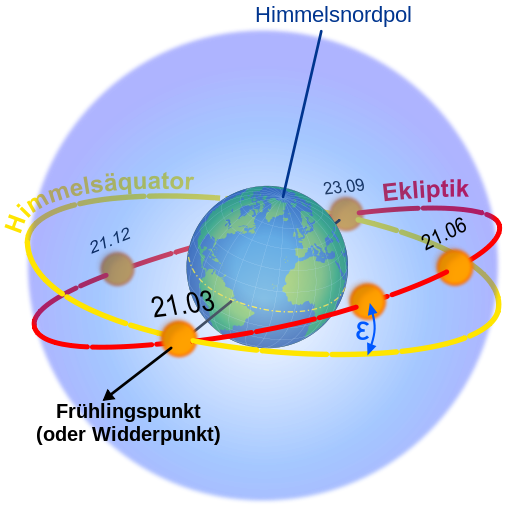
\includegraphics[scale=0.3]{./Bilder/Ecliptic.png}\hfill
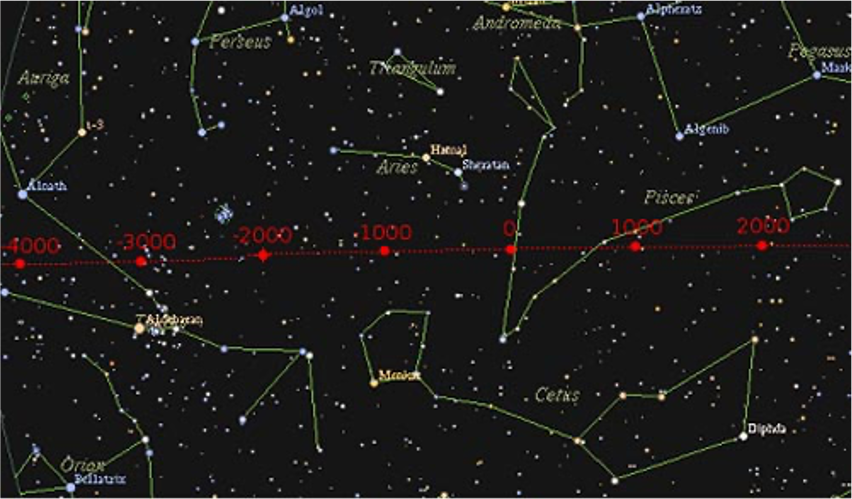
\includegraphics[scale=0.6]{./Bilder/Fr-Punkt.png}
\caption{\label{fig_Fruehlingspunkt}%
(links) Der Fr\"uhlingspunkt als der Schnittpunkt zwischen dem Himmels\"aquator und
der Ekliptik. (rechts) Der Fr\"uhlingspunkt in den letzten Jahrtausenden. W\"ahrend der 
Fr\"uhlingspunkt heute (im Jahr 2023)
im Sternbild Fische (Pisces) steht, stand er vor rund 2500 Jahren im Sternbild
Widder (Aries). Und in einigen Jahrhunderten wird er im Sternbild Wassermann stehen.
(links \cite{Wiki_Fruehling}, rechts \cite{Rocket})}
\end{figure}
 
 Die beiden Gro\ss kreise - Himmelsekliptik und Himmels\"aquator - schneiden sich in zwei
 Punkten. Der Fr\"uhlingspunkt ist definiert als der Schnittpunkt, bei dem sich die Sonne
 von S\"uden nach Norden durch die \"Aquatorialebene bewegt, beim Herbstpunkt bewegt sie sich von Nord
 nach S\"ud durch die \"Aquatorialebene. Derzeit liegt der Fr\"uhlingspunkt im Sternbild Fische. In einigen
 hundert Jahren wird er in das Sternbild Wassermann eintreten, und in babylonischer Zeit, als die Tierkreiszeichen
 benannt wurden, befand sich der Fr\"uhlingspunkt im Sternbild Widder. Aus diesem Grunde hei\ss t er 
 auch heute noch gelegentlich Widderpunkt (siehe Abb\ \ref{fig_Fruehlingspunkt}, rechts).
 
 Durch die Angabe der genannten Bezugsgr\"o\ss en - Himmelsnordpol, Himmels\"aquator und
 Fr\"uhlingspunkt auf dem Himmels\"aquator - k\"onnen wir ein Koordinatensystem f\"ur den Himmel, also
 ein sph\"arisches Koordinatensystem konstruieren.
Dazu definiert man L\"angengrade - halbe Gro\ss kreisb\"ogen vom 
 Himmelsnordpol zum Himmelss\"udpol (auch als Stundenlinien bezeichnet) -\index{Stundenlinie} 
 und Breitengrade - Kreisb\"ogen, deren Punkte unter einem konstanten
 Winkel relativ zum Himmelsnordpol stehen. Die Breitengrade werden durch die sogenannte
 Deklination\index{Deklination} 
 gekennzeichnet: Dies ist der Winkel $\delta$ von der \"Aquatorialebene zu einem Himmelsobjekt
 entlang eines L\"angengrads. Die Deklination wird als Winkel zwischen $+90^\circ$ und $-90^\circ$ 
 (Nord- bzw.\ S\"udrichtung) angegeben. Genauere Bezeichnungen verwenden meist Bogenminuten,
 Bogensekunden und dann Nachkommastellen. Der L\"angengrad wird ausgehend vom Fr\"uhlingspunkt
meist in Stundenwinkeln angegeben: der volle Himmels\"aquator wird entgegen dem Uhrzeigersinn in 
24 Stundenwinkel eingeteilt, entsprechend sind genauere Bezeichnungen in Minuten und Sekunden.
Diesen Stundenwinkel bezeichnet man als Rektazension.\index{Rektazension}
Beispielsweise hat Arkturus, einer der hellsten Sterne des Nordhimmels im Sternbild Bootes (B\"arenh\"uter), 
die Rektazension $14^{\rm h}\,15^{\rm m}\,39,67207^{\rm s}$ und die Deklination $+19^\circ\, 10'\, 56,6730''$,
bezogen auf die Epoche J2000. 

\subsection{Ekliptische Koordinaten}

Statt des Himmels\"aquators und dem dazu senkrecht stehenden Himmelsnordpol kann man 
auch\index{Ekliptische Koordinaten}\index{Koordinaten!ekliptische}
den Gro\ss kreis zur Ekliptik der Sonne und einen dazu senkrecht stehenden Punkt am Himmel
als Koordinatensystem w\"ahlen. Statt der Rektazension und der Deklination verwendet man hier den
ekliptischen L\"angengrad und den ekliptischen Breitengrad. Beide werden in Winkelma\ss en angegeben,
wobei der ekliptische L\"angengrad eine Winkeleinteilung der Ekliptik in $360^\circ$ angibt und der ekliptische
Breitengrad im Bereich zwischen $+90^\circ$ (ekliptischer Nordpol) bis $-90^\circ$ (ekliptischer S\"udpol) liegt. 
Auf der Himmelsekliptik wird ebenfalls der Fr\"uhlingspunkt als
Nullpunkt f\"ur die L\"angengrade ausgezeichnet. 

Dieses Koordinatensystem wird seltener verwendet (wegen der Bewegung vieler Planeten in der
N\"ahe der Ekliptik findet es zur Beschreibung solcher Himmelsobjekte schon mal Verwendung), sodass
wir hier nicht weiter darauf eingehen.

\subsection{Galaktische Koordinaten}

Schlie\ss lich verwendet man in der Astronomie auch gelegentlich das 
galaktische Koordinatensystem.\index{Galaktische Koordinaten}\index{Koordinaten!galaktische}
Als ausgezeichneter Referenzkreis dient ein Gro\ss kreis am Himmel, der mehr oder weniger durch
die Ebene der Milchstra\ss e, also die Sterne in der Ebene unserer Galaxie, ausgezeichnet ist. 
Der Ursprung des dreidimensionalen Koordinatensystems ist die Sonne, das Zentrum der
Galaxie (im Sternbild Sch\"utzen) dient als Referenzpunkt auf der galaktischen Ebene. 
Der galaktische Nordpol steht senkrecht auf der galaktischen Ebene und liegt im mittleren oberen Teil des Sternbilds
Haar der Berenike (Coma Berenices),\index{Haar der Berenike}\index{Coma Berenices} 
n\"ordlich des Sternbilds Jungfrau und rund $30^\circ$ s\"udlich (also
vom Nordpol weggerichtet) des Gro\ss en Wagens. 

Von der Erde aus betrachtet handelt es sich zwar um ein sph\"arisches Koordinatensystem, es
dient aber auch bei bekannten Entfernungen zu Himmelsobjekten als dreidimensionales Koordinatensystem
zur Lagebezeichnung von Objekten innerhalb unserer Galaxie.  

\section{Sternbilder}

Wie schon erw\"ahnt wurden von der IAU (International Astronomical Union) 88 Sternbilder mit ihren
Grenzen als verbindlich festgelegt (siehe Abb.\ \ref{fig_Sternbilder}).\index{Sternbild} 
Die Grenzen bestehen aus Kreisb\"ogen zu konstanter Deklination bzw.\
konstanter Rektazension - bilden somit in einer \"aquatorialen Zylinderprojektion 
senkrechte und waagerechte Linien - und umranden jeweils eine Fl\"ache.\footnote{Das Sternbild Schlange (Serpens) 
besteht als einziges Sternbild aus zwei\index{Schlange (Sternbild)}\index{Serpens caput/Serpens cauda} 
Fl\"achen, die man als Schlangenkopf (Serpens caput) und
Schlangenschwanz (Serpens cauda) bezeichnet. Die beiden Teile befinden sich rechts und links vom Sternbild 
Schlangentr\"ager (Ophiuchus)\index{Schlangentr\"ager}\index{Ophiuchus} 
und sind in den Sommermonaten am Abend in s\"udwestlicher Richtung gut zu sehen.} 
In der Summe \"uberdecken diese Fl\"achen die gesamte Himmelskugel. 

\begin{figure}[htb]
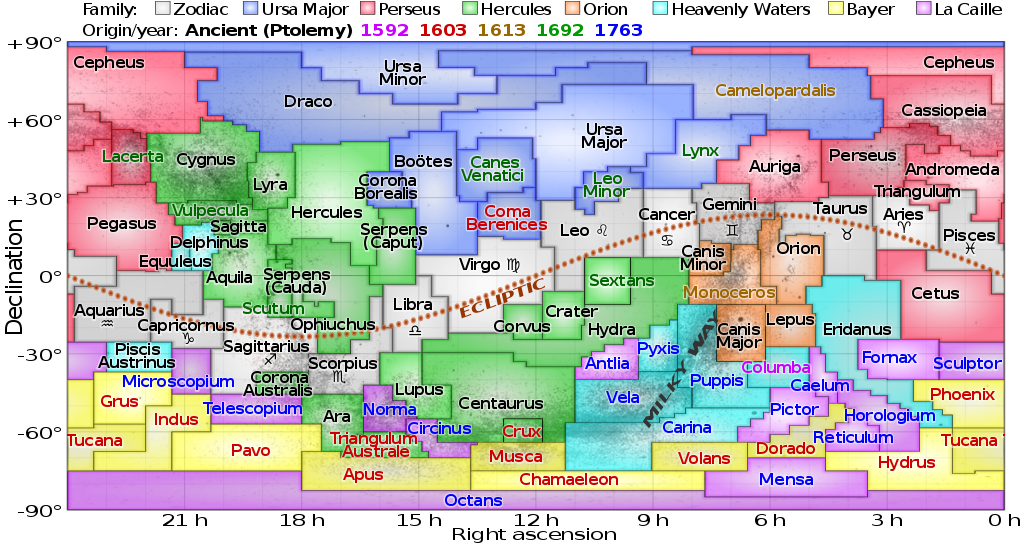
\includegraphics[scale=0.42]{./Bilder/Constellations.png}  % besser ist scale=0.42, sofern m�glich
\caption{\label{fig_Sternbilder}%
Die 88 Sternbilder in der \"Aquatorialdarstellung. Die Hintergrundfarben beziehen sich auf verschiedene Gruppen
von Sternbildern, insbesondere handelt es sich bei den grau hinterlegten Sternbildern um die klassischen
Tierkreiszeichen. In schwarzer Schrift sind die klassischen Sternbilder des Ptolem\"aus bezeichnet, andere
Farben kennzeichnen Sternbilder, die erst in sp\"aterer Zeit hinzugekommen sind. (aus \cite{Sternbilder})}
\end{figure}

In manchen Sternbildern sind mit blo\ss em Auge kaum markante Sterne zu sehen. 
Dass man diesen Fl\"achen trotzdem 
ein eigenes Sternbild zugeordnet hat liegt daran, dass man mit der Erfindung des Fernrohrs unz\"ahlige Objekte
entdeckte, die mit blo\ss em Auge nicht erkennbar sind. Um den Ort dieser Objekte am Himmel grob angeben
zu k\"onnen, hat man den gesamten Himmel mit Sternzeichen \"uberdeckt. Auf der Webseite des 
\textit{Strasbourg astronomical Data Center} \cite{IAU_Daten}
findet man die exakten Grenzen (bezogen auf das Besseljahr 1875)
aller Sternbilder. Sehr wenige Sternbilder (z.B.\ der Sextant - Sextans - 
s\"udlich vom Sternbild L\"owen) bilden\index{Sextant (Sternbild)}
ein einfaches Quadrat. Eines der komplexesten Sternbilder ist das Sternbild 
Drachen (Draco) mit rund\index{Drachen (Sternbild)}\index{Draco}
50 Grenzlinien, das sich zwischen dem kleinen und gro\ss en B\"aren halb um den Polarstern windet.   

Jedes Sternbild besitzt einen lateinischen Namen und eine Abk\"urzung mit drei Buchstaben: z.B.\ UMa f\"ur 
Ursa Major\index{Ursa Major}
 - Gro\ss e B\"arin (im Deutschen meist als Gro\ss er B\"ar bezeichnet) oder Sgr f\"ur 
 Sagittarius - Sch\"utze.\index{Sagittarius}\index{Sch\"utze (Sternbild)}
Diese Nomenklatur geht auf Henry Norris Russell zur\"uck (nach dem auch das Hertzsprung-Russell-Diagramm
benannt ist), der diese Bezeichnungen 1922 vorschlug. Innerhalb eines Sternbilds werden die hellsten Sterne
meist durch einen griechischen Buchstaben sowie den Genitiv des lateinischen Sternbildnamens 
bezeichnet, wobei sich in
der Regel die Reihenfolge $\alpha$, $\beta$, etc.\ nach der Helligkeit der Sterne richtet. Allerdings gilt diese Regel
nicht streng: Im Sternbild Ursa Major (Gro\ss er B\"ar) scheint sich die Reihenfolge eher an der Reihenfolge in
dem Asterismus Gro\ss er Wagen zu orientieren als an der Helligkeit. So ist $\alpha$ Ursae Majoris der zweithellste
Stern in diesem Sternbild, wohingegen $\epsilon$ Ursae Majoris der hellste ist. Wenn das griechische Alphabeth
durchgelaufen ist, verwendet man oft lateinische Buchstaben und anschlie\ss end Zahlen. 

Bei Doppel- oder Dreifachsternsystemen bezeichnet man die Sterne dieses Systems nach dem Namen mit einem
angeh\"angten Gro\ss buchstaben.
So ist $\alpha$ Centauri ein\index{alpha@$\alpha$ Centauri} 
Dreifachsternsystem, wobei $\alpha$ Centauri A und $\alpha$ Centauri B
vergleichsweise helle Sterne sind, wohingegen es sich bei\index{Proxima Centauri} 
$\alpha$ Centauri C (auch Proxima Centauri genannt, da
es sich mit 4,26 Lichtjahren um den uns n\"achsten Stern nach der Sonne handelt) um einen roten Zwerg handelt, der
nur in einem guten Fernrohr sichtbar ist. Oft verwendet man auch die Abk\"urzungen, beispielsweise $\alpha$ Cen A. 

Die hellsten Sterne haben eigene Namen, die meist aus der Antike stammen. Auf \cite{Wiki_hellste} findet man
eine Liste der 100 hellsten Sterne mit ihren Namen, Helligkeiten, Magnituden, offiziellen Bezeichnungen sowie
ihrer Rektazension und Deklination. Etwas umfangreichere Listen findet man auf \cite{brightest}.         

\section{Tierkreiszeichen}

Tierkreiszeichen\index{Tierkreiszeichen} 
sind Sternzeichen, die auf der Ekliptik liegen, d.h.\ vor denen von der Erde aus betrachtet 
die Sonne im Laufe eines Jahres einmal steht (siehe Abb.\ \ref{fig_Sternbilder}). 
Streng genommen sollte man zwischen den sogenannten
siderischen Tierkreiszeichen (die man besser als Sternbilder der Ekliptik bezeichnet) 
und den tropischen Tierkreiszeichen unterscheiden. 

Die siderischen Tierkreiszeichen oder auch Ekliptiksternbilder
sind die Sternzeichen, wie sie von der IAU definiert wurden und die auf der Ekliptik liegen. Sie unterteilen den
Vollkreis der Ekliptik in nicht immer exakt gleich lange Anteile von ungef\"ahr $30^\circ$. Allerdings gibt es hier schon 
eine Besonderheit: Das Sternbild des Schlangentr\"agers (Ophiuchus) \"uberdeckt zwischen dem Sternbild 
Skorpion (Scorpio) und dem Sternbild Sch\"utzen (Sagittarius) mit seinem unteren Rand ebenfalls einen 
Teil der Ekliptik. Die beiden Anteile der Ekliptik zum Skorpion und zum Schlangentr\"ager ergeben zusammen
einen Abschnitt von ungef\"ahr $30^\circ$, wobei der Anteil des Schlangentr\"agers deutlich gr\"o\ss er als der des
Skorpions ist. Der Schlangentr\"ager z\"ahlt aber in der Tradition nicht zu den Tierkreiszeichen. In manchen Listen
wird der Schlangengtr\"ager heute als 13.\ Tierkreiszeichen hinzugez\"ahlt, insbesondere wenn man von den
siderischen Tierkreiszeichen bzw.\ Ekliptiksternbildern spricht. 

Dem gegen\"uber gibt es die tropischen Tierkreiszeichen. Sie unterteilen die Ekliptik in zw\"olf exakt gleich gro\ss e
Anteile von $30^\circ$ und tragen dieselben Bezeichnungen wie die siderischen Tierkreissternbilder. 
Allerdings hat sich aufgrund der Pr\"azission der Erde der Fr\"uhjahrspunkt im Verlauf der Zeit verschoben. Vor etwas
\"uber 2500 Jahren, als die Bezeichnungen der Tierkreiszeichen in Babylonien entstanden sind, 
befand sich der Fr\"uhjahrspunkt im
Sternbild Widder, weshalb man ihn auch heute noch manchmal als Widderpunkt bezeichnet. Auf diese Einteilung
der Ekliptik in zw\"olf gleiche Teile bezieht sich auch heute noch die Astrologie: Die astrologischen Tierkreiszeichen 
beginnen am 21.\ M\"arz mit dem Zeichen Widder und schreiten in nahezu gleichen zeitlichen Abst\"anden um jeweils
$30^\circ$ voran.\footnote{Die Wendepunkte und \"Aquinoktien definieren jeweils gleiche Abschnitte von $90^\circ$.
Wegen der elliptischen Bahn und der damit verbundenen ungleichen Geschwindigkeit der Erde um die Sonne 
sind die zugeh\"origen r\"aumlichen und zeitlichen Abschnitte jedoch nicht
exakt gleich lang.} Heute liegt der Fr\"uhjahrspunkt im Sternbild Fische, und in einigen Jahrhunderten wird er
ins Sternbild Wassermann gewandert sein. Das bedeutet, derzeit sind die tropischen und die 
siderischen Tierkreiszeichen gegeneinander um ein Zeichen verschoben: Am 21.\ M\"arz, 
wenn das tropische Tierkreiszeichen Widder
beginnt, befindet sich die Sonne im Sternzeichen Fische.  

Unter dem Zodiak,\index{Zodiak} 
fr\"uher oft synonym zu Tierkreiszeichen verwendet, versteht man heute ein Band von rund 
$\pm 10$ Grad um die Ekliptik, in der sich die meisten Planetenbahnen sowie die Bahn des Mondes bewegen. Auch 
der Zodiak ist in zw\"olf exakt $30^\circ$ umfassende Bereiche unterteilt und richtet sich insofern nach den
tropischen Tierkreiszeichen. 

Gew\"ohnlich beginnt man die Reihe der Tierkreiszeichen mit dem\index{Widder (Sternbild)}\index{Aries} 
Widder (Aries), in dem vor rund 2500 Jahren der 
Fr\"uhlingspunkt lag. In aufsteigender Rektazension, also entgegen dem Uhrzeigersinn, folgen die Tierkreiszeichen
Stier (Taurus), Zwillinge (Gemini), Krebs (Cancer), L\"owe (Leo), Jungfrau (Virgo), Waage (Libra), Skorpion (Scorpius),
Sch\"utze (Sagittarius), Steinbock (Capricornus), Wassermann (Aquarius) und Fische (Pisces), wobei man 
im Zusammenhang mit den Ekliptiksternbildern 
zwischen den Skorpion und den Sch\"utzen noch den Schlangentr\"ager als 13.\ Tierkreissternbild einf\"ugt. 

\section{Asterismen}

Asterismen\index{Asterismus} 
sind einzelne Gruppen von Sternen, die ein markantes Muster zeigen. Bekannte
Beispiele sind der gro\ss e und kleine Wagen in den Sternbildern Ursa Major und Ursa Minor mit jeweils
sieben Sternen, wobei man bei nicht optimalen Sichtverh\"altnissen vom kleinen Wagen oft nur drei
Sterne sieht, oder auch das Himmels-W der Kassiopeia aus f\"unf Sternen. Ein weiteres Beispiel
(bekannt unter anderem aus dem Film \glqq Men in Black\grqq) ist der G\"urtel des Orion, bestehend
aus drei hellen Sternen in einer Reihe. 

Ein Asterismus kann auch aus Sternen zu verschiedenen Sternbildern bestehen. Beispiele
hier sind das Fr\"ulingsdreieck,\index{Fruehlingsdreieck@Fr\"uhlingsdreieck} 
bestehend aus Spica (Sternbild Jungfrau - Virgo), Arktur (Sternbild 
B\"arenh\"uter - Bootes) und Regulus (Sternbild L\"owe - Leo), oder auch das 
Sommerdreieck,\index{Sommerdreieck}
bestehend aus Wega (Sternbild Leier - Lyra), Altair (Sternbild Adler - Aquila) und Deneb (Sternbild Schwan - Cygnus). 
Hierbei handelt es sich jeweils um eine Gruppe von drei besonders hellen Sternen, die man im
Fr\"uhjahr bzw.\ im Sommer am Abendhimmel sehen kann. Ein weiteres Beispiel ist das 
Wintersechseck,\index{Wintersechseck}
bestehend aus den Sternen Capella (Sternbild Fuhrmann - Auriga), Aldebaran (Sternbild Stier - Taurus), 
Rigel (Sternbild Orion), Sirius (Sternbild Gro\ss er Hund - Canis Major), Prokyon (Sternbild Kleiner Hund -
Canis Minor) und Pollux (Sternbild Zwillinge - Gemini). Diese Sterngruppen erstrecken sich teilweise
\"uber einen gro\ss en Teil des Nachthimmels. 

Es gibt aber auch sehr kleine Asterismen, die man mit blo\ss em Auge kaum aufl\"osen kann, wohl
aber mit einem einfachen Fernglas: Ein Beispiel ist der\index{Kleiderb\"ugel (Asterismus)} 
\glqq Kleiderb\"ugel\grqq\ im Sternbild Fuchs (Vulpecula,
zwischen den Sternbildern Adler und Schwan gelegen). Der Asterismus besteht aus 10 Sternen, von denen
sechs nahezu auf einer Geraden liegen, plus vier Sterne, die in der Mitte \"uber dieser Geraden einen
Dreiviertelkreis bilden. Insgesamt erscheint diese Konfiguration, die offiziell den 
Namen Collinder 399 tr\"agt,\index{Collinder 399}
wie ein Kleiderb\"ugel.   


\begin{thebibliography}{99}
\bibitem{IAU_Daten} Strasbourg astronomical Data Center, Grenzen der Sternbilder:\\
      \url{https://vizier.cds.unistra.fr/vizier/VizieR/constellations.htx}.   
\bibitem{Rocket} Rocket Site \glqq Wann beginnt das Zeitalter des Wassermanns?\grqq\
               \url{https://damthoitrang.org/de/wann-beginnt-das-zeitalter-des-wassermanns/}      
\bibitem{Sternbilder} aus Wikipedia \glqq Zodiac\grqq, Quelle: 
      \url{http://svs.gsfc.nasa.gov/vis/a000000/a003500/003572}, Autor: Cmglee, Timwi, NASA. 
\bibitem{Wiki_Fruehling} Wikipedia \glqq \"Aquinoktium\grqq, 
                 \url{https://commons.wikimedia.org/wiki/File:Ecliptic.svg}
\bibitem{Wiki_hellste} Wikipedia \glqq Liste der hellsten Sterne\grqq: 
      \url{https://de.wikipedia.org/wiki/Liste_der_hellsten_Sterne} 
\bibitem{brightest} Listen heller Sterne: \url{http://stars.astro.illinois.edu/sow/bright.html} (Webseite von
      Jim Kahler, die 172 hellsten Sterne) und
       \url{http://www.atlasoftheuniverse.com/stars.html} (Atlas of the Universe; die 300 hellsten Sterne). 
\end{thebibliography}

\end{document}

